\chapter{Experimente}
\label{cha:experimente}

\section{Vereinfachte Kalibrierung}
\label{sec:vereinfachtekalib}

Eine andere M"oglichkeit, als die Kalibrierung mittels eines Schachbretts, wie sie in \ref{sec:kalibrierung} erl"autert wurde, ist mit Hilfe eines rechteckigen Kalibrierobjektes. In unserem Fall handelt es sich, wie in \ref{fig:klammern} zu sehen ist, um die Verpackung von Heftklammern.
 
\begin{figure}[H]
	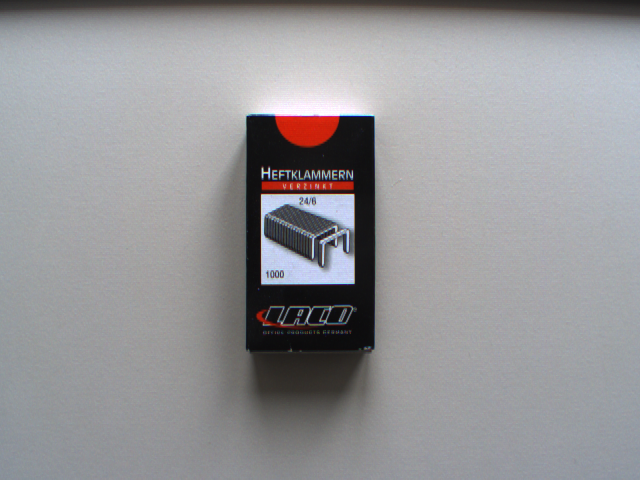
\includegraphics[scale=0.5]{bilder/experimentcalib}
	\caption[Kalibrierobjekt]{Kalibrierobjekt}
	\label{fig:klammern}
\end{figure}

\newpage

\noindent Die Formel zur Berechnung der Brennweite $f_x$ und $f_y$ ergibt sich aus den Formeln

\begin{equation}
f_x=\frac{\Delta x'}{x}z
\end{equation}

und

\begin{equation}
f_y=\frac{\Delta y'}{y}z
\end{equation}

\noindent bei $\Delta x$ und $\Delta y$ handelt es sich um die jeweiligen Seitenl"angen des Kalibrierobjekts.\newline
$\Delta x'$ und $\Delta y'$ sind die L"angen der Seiten des Kalibrierobjekts in Pixelwerten. $z$ ist der Abstand zwischen Linse und Objekt \cite{PCV} \cite{CVF}.

\begin{figure}[H]
	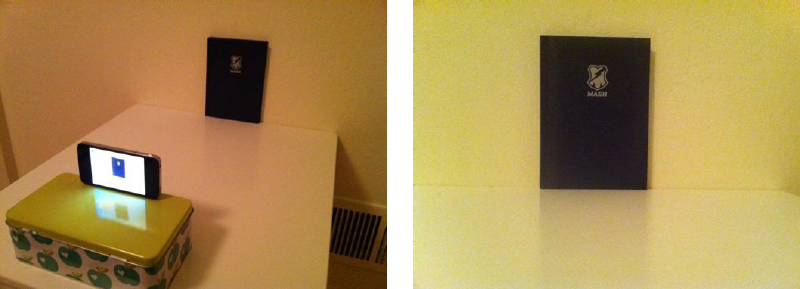
\includegraphics[scale=1.0]{bilder/simple_calib}
	\caption[Vereinfachte Kalibrierung]{Vereinfachte Kalibrierung}
	\small Quelle: Solem 2012
	\label{fig:simplecalib}%
\end{figure}

\noindent Wie in \ref{fig:simplecalib} zu sehen ist, muss das Kalibrierobjekt senkrecht auf eine planare Oberfl"ache gestellt werden. So auch die Kamera. Die Kamera muss dann so ausgerichtet werden, dass das Objekt im Bild genau zentriert und entlang der Bildzeilen und -spalten ausgerichtet ist \cite{CVF}.\newline
Obwohl diese Kalibrierung sehr ungenau erscheint, wurde dennoch ein relativ geringer Reprojection-Error errechnet. Der Fehler bei der in \ref{sec:kalibrierung} beschriebene Methode war jedoch besser.

\section{Fehlerfortpflanzung}
\label{sec:fehlerfortpflanzungtiefen}

Bei der Tiefenberechnung mit Hilfe eines Stereokamerasystems wird die Raumposition nicht gemessen, sondern aus den beiden vom Kamerasystem erfassten Bildern berechnet. Dazu wird der gleiche Raumpunkt in beiden Bildern detektiert. Die räumliche Rekonstruktion ist im Stereonormalfall besonders einfach, da die beiden Kameras keine Rotation zueinander aufweisen. Dadurch vereinfachen sich die allgemeinen Formeln zur räumlichen Rekonstruktion \cite{frz}

\begin{equation}
x = x_{0} + (z - z_{0})\frac
{r_{11}(x'-x_{0}') + r_{12}(y'-y_{0}')-r_{13}f}
{r_{31}(x'-x_{0}') + r_{32}(y'-y_{0}')-r_{33}f}
\end{equation}

\begin{equation}
y = y_{0} + (z - z_{0})\frac
{r_{21}(x'-x_{0}') + r_{22}(y'-y_{0}')-r_{23}f}
{r_{31}(x'-x_{0}') + r_{32}(y'-y_{0}')-r_{33}f}
\end{equation}

\noindent zu\newline
\noindent Rechtes Bild:
\begin{equation}\label{eq:one}
x = -z \frac{x'_{1}}{f}
\end{equation}
\begin{equation}\label{eq:two}
y = -z \frac{y'_{1}}{f}
\end{equation}

\noindent Linkes Bild:
\begin{equation}\label{eq:three}
x = B-z \frac{x'_{2}}{f}
\end{equation}
\begin{equation}\label{eq:four}
y = -z \frac{y'_{2}}{f}
\end{equation}

\noindent Aus den vereinfachten Formeln \ref{eq:one}, \ref{eq:two}, \ref{eq:three} und \ref{eq:four}, ist ersichtlich, dass ein Raumpunkt in beiden Bildern die gleiche $y$-Koordinate aufweist, sich jedoch normalerweise in der $x$-Koordinate unterscheidet. Diese Differenz wird als $x$-Parallaxe 
$\rho_{x} = x_{1} - x_{2}$ oder Disparität $d$ bezeichnet.\newline
\noindent Durch Gleichsetzen der Formeln \ref{eq:one} – \ref{eq:four} für linkes und rechtes Bild, erhält man folgende Formel zur Berechnung der Tiefeninformation:

\begin{equation}\label{eq:tiefe}
z = -\frac
{f*B}
{x'_{1}-x'_{2}}
=
-\frac
{f*B}
{\rho x'}
\end{equation}

\noindent Da die Brennweite f und der Abstand der beiden Kameras zueinander (Baseline $B$) konstant sind, ist die Entfernung allein von der $x$-Parallaxe abhängig. Dabei ist ein Punkt näher, je größer die Parallaxe ist. \newline
Die Formel \ref{eq:tiefe} wurde mit folgendem Experiment validiert:


\begin{figure}[!htb]
	\minipage{0.32\textwidth}
	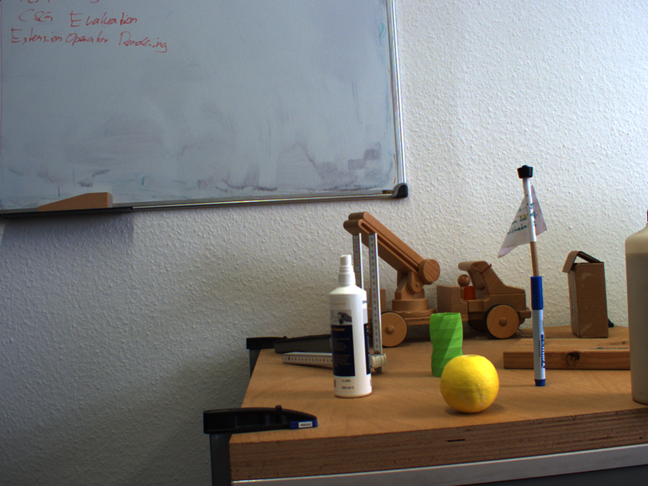
\includegraphics[width=\linewidth]{bilder/depth_left}
	\caption{Tiefe links}\label{fig:depthleft}
	\endminipage\hfill
	\minipage{0.32\textwidth}
	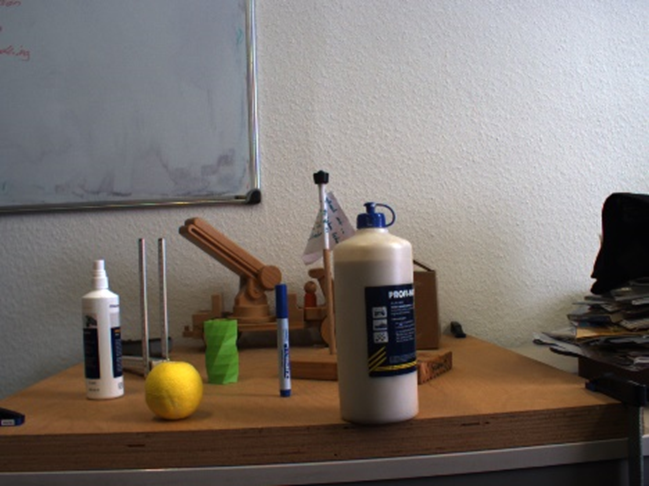
\includegraphics[width=\linewidth]{bilder/depth_right}
	\caption{Tiefe rechts}\label{fig:depthright}
	\endminipage\hfill
	\minipage{0.32\textwidth}%
	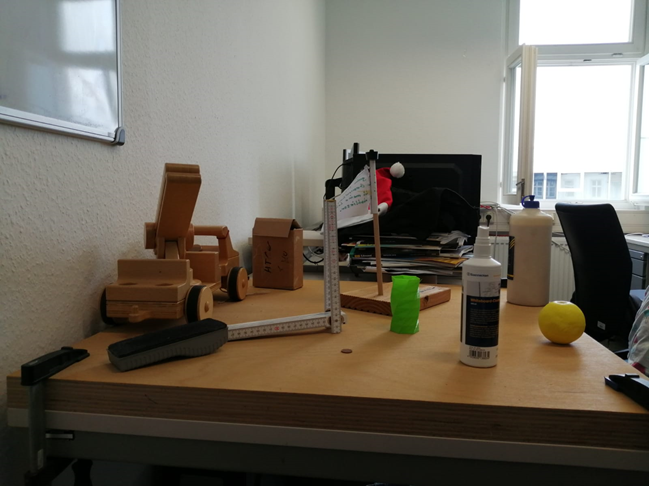
\includegraphics[width=\linewidth]{bilder/depth_side}
	\caption{Tiefe seitlich}\label{fig:depthside}
	\endminipage
\end{figure}

\noindent Mit dem Stereo-System wurden zwei Aufnahmen einer Szene aufgenommen (\ref{fig:depthleft} und \ref{fig:depthright}). Auf dem seitlichen Bild \ref{fig:depthside} sieht man die tats"achliche Tiefe der Objekte im Bild.

\begin{figure}[!htb]
	\minipage{0.48\textwidth}
	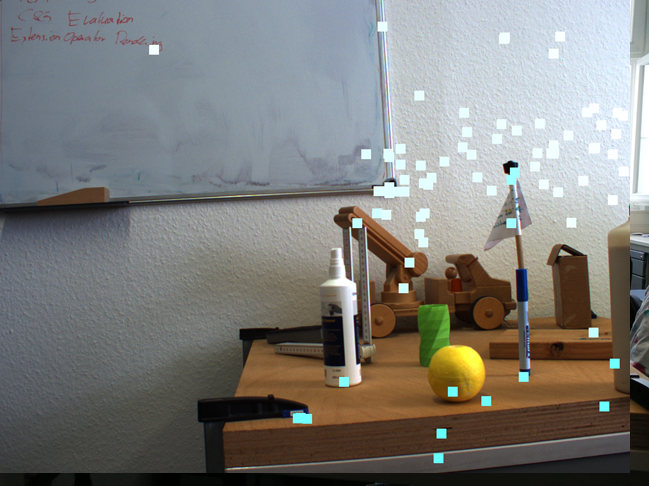
\includegraphics[width=\linewidth]{bilder/depth_result}
	\caption{Tiefeninformation Punkte}\label{fig:depthpoints}
	\endminipage\hfill
	\minipage{0.48\textwidth}
	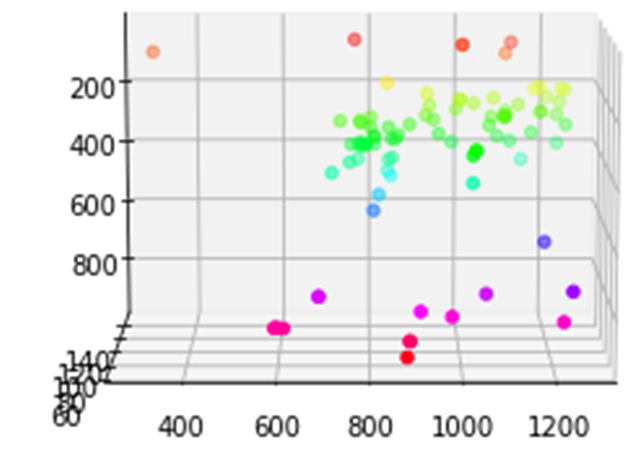
\includegraphics[width=\linewidth]{bilder/depth_coord}
	\caption{Tiefeninformation 3D-Plot}\label{fig:depthplot}
	\endminipage\hfill
\end{figure}

\noindent Auf den zwei Bildern der Szene wurden hier vorerst h"andisch, dann mittels des SIFT-Algorithmus Referenzpunkte ermittelt, zu denen die Tiefe berechnet werden sollte.\newline
\noindent Mittels eines selbst geschriebenen Algorithmus, der Werte mit großem $z$ wei"slich und Werte mit kleinem $z$ hellblau einf"arbt, kann die Informationen zur Tiefe auf einem Bild dargestellt werden. In \ref{fig:depthpoints} kann man gut erkennen, dass Objekte, die n"aher an der Kamera stehen, mit einem hellen Blau markiert sind. Objekte, die weiter entfernt sind, mit einem wei"slichem Farbton.\newline
\noindent Dieses Verfahren der indirekten Bestimmung der Tiefeninformationen ist jedoch anfällig für Messfehler in den Bildpositionen. Die Fehlerfortpflanzung über die Werte $x$, $y$ und $z$ wird mit Hilfe des Gaußschen Fehlerfortpflanzungsgesetzes, welches den Einfluss mehrerer fehlerbehafteter Eingangsgrößen auf eine zu schätzende Ausgangsgröße beschreibt, berechnet.
Wird die Varianz der Ausgangsgröße $y$ über die fehlerbehafteten Eingangsgrößen $x_{1}$ bis $x_{n}$  abgeschätzt, lautet die allgemeine Form des Gaußschen Fehlerfortpflanzungsgesetzes:

\begin{equation}
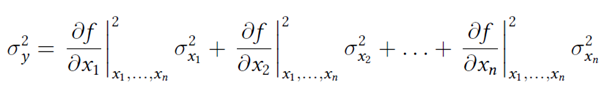
\includegraphics[scale=1.0]{bilder/formel3}
\end{equation}

\noindent Wendet man dieses Gesetz auf die Formeln \ref{eq:one} - \ref{eq:tiefe} an, erhält man folgende Fehlerabschätzung für die Größen $z$, $y$ und $z$ unter der Annahme, dass die Brennweite $f$ und die Baseline $B$ fehlerfrei sind \cite{frz}:

\begin{equation}\label{eq:fourone}
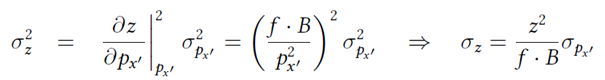
\includegraphics[scale=1.0]{bilder/fourone}
\end{equation}

\begin{equation}\label{eq:fourtwo}
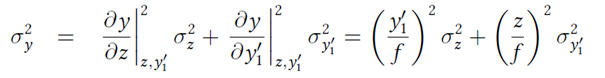
\includegraphics[scale=1.0]{bilder/fourtwo}
\end{equation}

\begin{equation}\label{eq:fourthree}
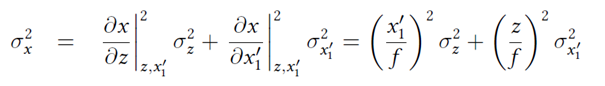
\includegraphics[scale=1.0]{bilder/fourthree}
\end{equation}


\section{Genauigkeitsabschätzung des Systems}
\label{sec:genauigkeit}

Zur Genauigkeitsbeurteilung haben wir drei Mal das gleiche Objekt in jeweils einem anderen Abstand zum Stereosystem aufgenommen. Dabei erhielten wir folgende Resultate:

\begin{center}
	\begin{tabular}{  l | l | l }
		\hline
		Gemessener Abstand [cm] & Berechneter Abstand [cm] & Differenz [cm] \\ \hline
		37 & 31,05 & 5,95 \\ \hline
		54 & 48,78 & 5,22 \\
		100 & 96,81 & 3,19 \\
	\end{tabular}
\end{center}

\noindent Überraschenderweise nimmt der Fehler mit zunehmender Distanz in diesem Fall ab. Auf Grund der Fehlerformel für $z$ (s. \ref{eq:fourone}) war zu erwarten, dass der Fehler in der Tiefe quadratisch mit der Distanz wächst, was hier jedoch nicht der Fall ist. Auch bei der händischen Tiefenberechnung mit zwei rektifizierten Schachbrettmustern trat ein Phänomen auf, wobei die Disparität von Punkten links in den beiden Bildern nach rechts stark zunahm, obwohl die Punkte in der gleichen Entfernung zur Kamera waren.\newline
\noindent Dies ist auch die Ursache, weshalb keine ausführliche Fehlerfortpflanzungsrechnung für unser System durchgeführt wurde, da bereits a priori absehbar war, wenig aussagekräftige Ergebnisse zu erhalten. Leider konnten wir keine plausible Erklärung für dieses Verhalten finden, die einzige Vermutung ist, dass etwas mit der Kalibrierung der Kameras nicht ganz in Ordnung ist, was dieses unerwartete Verhalten verursacht. Doch auch durch mehrmaliges Neukalibrieren konnte das Problem nicht behoben werden. Folgende Abbildung zeigt den Versuchsaufbau:

\begin{figure}[H]
	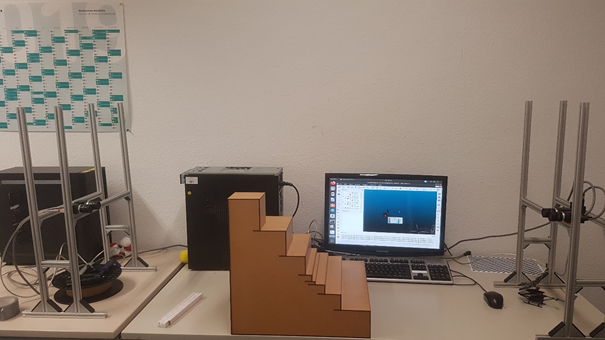
\includegraphics[scale=1.0]{bilder/abstandsmessung}
	\caption[Versuchsaufbau mit zwei Stereokamerasystemen und Objekt zur Abstandsmessung]{Versuchsaufbau mit zwei Stereokamerasystemen und Objekt zur Abstandsmessung}
	\label{fig:abstandsmessung}
\end{figure}

\section{Kalibrierung der beiden Stereokamerasysteme zueinander}
\label{sec:kalibbeide}

Durch Aufstellen eines zweiten identischen Stereokamerasystems gegenüber des bisher beschriebenen Systems (s. \ref{fig:abstandsmessung}) sollte die bisher in der generierten Punktewolke fehlende Rückansicht des Helikopters in der Punktewolke visualisiert werden. Auf diese Weise sollte also eine 360\degree \space 3D-Ansicht einer Szene generiert werden. Zunächst musste das zweite System entsprechend dem Vorgehen für das erste System kalibriert werden, bevor versucht werden konnte, die beiden System zueinander kalibrieren zu können, d.h. die Rotation und Translation der beiden Systeme zueinander zu bestimmen. Dies ist nötig, um die beiden separaten Punktewolken in ein gemeinsames Koordinatensystem überführen zu können.\newline
\noindent Zur Kalibrierung der beiden Systeme zueinander wurden mehrere verschiedene Ansätze in Betracht gezogen und getestet, um Korrespondenzpunkte im 3-dimensionalen Raum berechnen zu können. Mithilfe des Algorithmus ''Iterative Closest Points'' (ICP), welcher in \ref{sec:icp} erl"autert wird, sollten aus diesen 3D-Koordinaten die Rotation und Translation der Systeme zueinander bestimmt werden.\newline
\noindent Folgende Ansätze wurden in Betracht gezogen:

\begin{enumerate}
	\item Aufstellen eines Objektes mit mehreren Eckpunkten, die in beiden Systemen sichtbar sind mit anschließendem automatisiertem Auffinden von Korrespondenzpunkten mit Hilfe des rotationsresistenten Interest-Point-Detektors SIFT. Leider konnte der SIFT-Detektor nicht ausreichend korrekte Korrespondenzen in den beiden Aufnahmen der jeweils gewählten Referenzkameras der beiden Systeme detektieren, weshalb dieser Ansatz nicht weiterverfolgt wurde.
	
	
	\item Aufstellen eines Objektes mit mehreren Eckpunkten, die von beiden Systemen sichtbar sind. Aus den Aufnahmen sollten dann händisch die 2D-Koordinaten bestimmt und mit den Formeln 
	\ref{eq:one} - \ref{eq:tiefe} die 3D-Repräsentation des Punkts berechnet werden. Dieser Ansatz wurde wegen des hohen manuellen Aufwands zunächst nicht weiterverfolgt und als Notlösung, falls keine bessere Variante gefunden werden könnte, verbucht. 
	
	\item Als am vielversprechendsten erwies sich der Ansatz mit einem beidseitig bedruckten Schachbrettmuster zu kalibrieren. Dabei müssen die Eckpunkte des Schachbretts auf Vorder- und Rückseite möglichst exakt übereinander liegen. Dies muss bereits beim Druck berücksichtigt werden. Von dem Schachbrettmuster wird dann von beiden Systemen eine Aufnahme gemacht, diese rektifiziert und mit der aus der Kamera-Kalibrierung bereits bekannten OpenCV-Methode \textit{findChessBoardCorners} die Bildkoordinaten der Eckpunkte bestimmt. Aus diesen Bildkoordinaten können anschließend erneut mit den Formeln \ref{eq:one} - \ref{eq:tiefe} die 3D-Koordinaten mehrerer identischer Punkte für die beiden System berechnet werden. \newline 
	\noindent Mithilfe des ICP konnten die beiden 3D-Punktewolken der beiden Schachbrettmuster auch erfolgreich in eine Ebene transformiert werden, also die Translation der beiden Systeme zueinander bestimmt werden. Problematisch war jedoch die Bestimmung der Rotation, da die Punktewolken des Schachbretts nahezu symmetrisch sind und deshalb die 180\degree-Rotation nicht erkannt wird. Eigentlich müssten die jeweils oberen linken Ecken des Schachbrettmusters aus beiden Systemen aufeinander gemappt werden. Allerdings werden durch den ICP die linke obere Ecke des Schachbrettmusters aus dem linken System auf die rechte obere Ecke der Aufnahme aus dem rechten System abgebildet, wodurch keine Rotation erkannt wird. Bei einem anderen Setup der Stereosysteme zueinander wird das Schachbrettmuster nicht mehr gleichzeitig von beiden Systemen erkannt, weshalb das Problem dadurch ebenfalls nicht gelöst werden kann.
	
\end{enumerate}

\begin{figure}[H]
	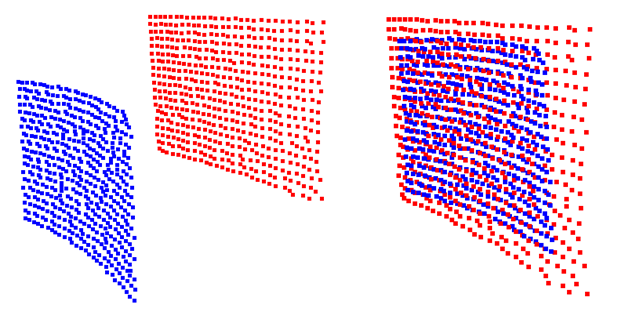
\includegraphics[scale=1.0]{bilder/icpresult}
	\caption[3D-Schachbrettmuster vor und nach der Transformation mit den Ergebnissen des ICP-Algorithmus]{3D-Schachbrettmuster vor und nach der Transformation mit den Ergebnissen des ICP-Algorithmus}
	\label{fig:icpresult}
\end{figure}

\subsection{ICP}
\label{sec:icp}

Der ICP Algorithmus ist eine Methode um zwei Punktewolken aneinander anzupassen \cite{icp1} \cite{icp2}.
Hierzu minimiert der Algorithmus den euklidischen Abstand $d$ von korrespondieren Punkten $q$ und $p$ in der Punktewolke:

\begin{equation}
d(q,p) = \sqrt{(q_{1}-p_{1})^{2} + ... + 
	(q_{n} -p_{n})^{2}}
\end{equation}

\noindent Die Zuordnung von Punktepaaren, um so korrespondieren Punkte zu finden, wird mittels des Nearest Neighbour Algorithmus vorgenommen. Dieser nimmt die beiden Punktewolken entgegen und liefert ein Feld mit Indizes zurück, welche die korrespondieren Punkte angeben. In unserem Projekt wird er in der optimierten Variante verwendet. Dieser beschreibt die Punktewolken in einer Baumstruktur.

\subsubsection{Ablauf}
\label{ss:ablauf}

Vorab wird angenommen, dass die Punktewolken näherungsweise aufeinander ausgerichtet wurden und als
initiale Transformation $T$ beschrieben wird. Diese Transformation wird auf die eine Punktewolke angewandt. Die daraus resultierende wird verwendet, um mit Hilfe des Nearest Neighbour Algorithmus die korrespondierenden Punktepaare zu finden. 
Als Gütemaß für die aktuelle Transformation wird die Summe der quadratischen Distanzen genommen. Diese gilt es zu minimieren. Aus diesen Ergebnissen werden dann die neuen Transformationsparameter abgeleitet \cite{icp3}:

\begin{equation}
T \leq argmin (\sum || d(q_{n}, p_{n}) || ^{2})
\end{equation}

\noindent Diese Schritte werden nun so oft wiederholt bis ein akzeptables Optimum gefunden ist. Der ICP Algorithmus terminiert also, sobald entweder ein definierter Schwellwert für das Gütemaß überschritten, oder eine definierte Anzahl an Iterationen erreicht wurde.
